\chapter{Conception Architecturale}
\label{chap:conception}

\section{Introduction}

Les exigences fonctionnelles, non fonctionnelles et la modélisation UML des besoins du système ont été formalisées au Chapitre~I (sections~1.3 et~1.4). Le présent chapitre se concentre exclusivement sur les décisions de conception architecturale issues de cette spécification. Il détaille la méthodologie de développement retenue (section~2.2), l'architecture logique multi-services (section~2.3), la modélisation mathématique du pipeline biométrique KYC (section~2.4), les processus métiers en notation BPMN (section~2.5) et enfin la modélisation statique du domaine (section~2.6). L'ensemble de la conception s'appuie sur les modélisations UML 2.5~\cite{fowler_uml_2003} et sur les processus métiers BPMN 2.0.
\section{Méthodologie et cadre de développement}
\label{sec:methodologie-globale}
\label{sec:methodologie}

La conception d'une plateforme distribuée requiert une démarche disciplinée. Nous avons retenu une approche itérative inspirée du Processus Unifié (\textsc{up}) allégé~\cite{kruchten_up_2004}, combinée à des itérations agiles de type \textit{Scrum} pour la réalisation. Le déroulement de nos itérations (sprints) est structuré dans le tableau~\ref{tab:sprints}, tandis que la segmentation de notre échantillon d'enquête et ses résultats clés sont synthétisés dans les tableaux~\ref{tab:profil-repondants} et~\ref{tab:resultats-enquete}.

Le recueil des besoins s'est articulé autour de trois axes méthodologiques.
\begin{enumerate}
  \item \textbf{Enquête utilisateurs :} Un questionnaire en ligne mené en mars 2026 et diffusé via les réseaux sociaux universitaires de Tlemcen et Oran auprès de 150 personnes a permis d'identifier les attentes prioritaires (sécurité, prix, disponibilité).
  \item \textbf{Étude comparative :} Une décomposition fonctionnelle approfondie des plateformes concurrentes a été réalisée afin de dégager les manques structurels du marché algérien.
  \item \textbf{Entretiens semi-directifs :} Des consultations ciblées et structurées ont été menées avec des conducteurs habitués aux longs trajets inter-wilayas.
\end{enumerate}

\subsection{Méthodologie de développement (cadre Scrum)}
\label{sec:scrum-planning}

Le développement a été organisé en \textbf{cinq sprints de deux semaines}, pilotés via \textit{Jira}. Les rôles Scrum ont été répartis de manière hybride au sein du binôme~: AHMED~BACHA (Product Owner / Développeur) et BELHORMA (Scrum Master / Développeur). Le tableau~\ref{tab:sprints} récapitule le déroulement effectif.

\begin{table}[!htbp]
\centering
\footnotesize
\renewcommand{\arraystretch}{1.3}
\begin{tabularx}{\textwidth}{|l|l|X|X|}
\hline
\rowcolor{rohlight}
\textbf{Sprint} & \textbf{Période} & \textbf{Objectif} & \textbf{Livrable} \\
\hline
\textbf{Sprint~1} & Sem.~1--2 & Fondation technique & Auth OTP, structure API, schéma BD, navigation mobile \\
\hline
\textbf{Sprint~2} & Sem.~3--4 & Fonctionnalités cœur & Publication/recherche de trajets, réservation, 69 wilayas \\
\hline
\textbf{Sprint~3} & Sem.~5--6 & Identité et confiance & Pipeline KYC (FastAPI), capture de la \gls{cin}, détection de vivacité \\
\hline
\textbf{Sprint~4} & Sem.~7--8 & Communication et paiement & Chat Socket.IO, suivi GPS, intégration CIB/Edahabia sandbox \\
\hline
\textbf{Sprint~5} & Sem.~9--10 & Stabilisation et admin & Dashboard React, tests Jest, correction de bugs, documentation \\
\hline
\end{tabularx}
  \caption{Déroulement des sprints Scrum}
  \label{tab:sprints}
\end{table}

Le Product Backlog initial comportait \textbf{42~User Stories} réparties sur les cinq sprints. Le taux de vélocité moyen s'est stabilisé à \textbf{18~story points par sprint} à partir du Sprint~3, après une phase d'apprentissage initiale. Les rétrospectives de chaque sprint ont conduit à trois ajustements majeurs~: (1)~le déplacement du module de tarification dynamique du Sprint~2 au Sprint~4 en raison de sa complexité algorithmique sous-estimée~; (2)~l'ajout du patron \textit{Factory} pour le paiement au Sprint~4 afin de faciliter l'intégration de nouvelles méthodes~; (3)~l'allocation de deux jours supplémentaires au Sprint~5 pour la stabilisation des tests d'intégration WebSocket.

\subsection{Enquête utilisateurs et étude de marché}
\label{sec:resultats-enquete}

Le questionnaire a recueilli 150 réponses exploitables entre le 1\textsuperscript{er} et le 20~mars~2026. Le tableau~\ref{tab:profil-repondants} résume le profil sociodémographique des répondants, et le tableau~\ref{tab:resultats-enquete} synthétise les résultats clés.

\begin{table}[!htbp]
\centering
\footnotesize
\begin{tabularx}{\textwidth}{|l|X|c|}
\hline
\rowcolor{rohlight}
\textbf{Critère} & \textbf{Détail} & \textbf{Proportion} \\
\hline
Tranche d'âge & 18--25 ans & 72\,\% \\
\hline
 & 26--35 ans & 19\,\% \\
\hline
 & 36+ ans & 9\,\% \\
\hline
Statut & Étudiants & 68\,\% \\
\hline
 & Salariés / indépendants & 32\,\% \\
\hline
Wilayas & Tlemcen, Oran, Alger, Sidi Bel Abbès, Aïn Témouchent & 84\,\% \\
\hline
Fréquence inter-wilayas & $\geq$ 1~trajet/semaine & 41\,\% \\
\hline
 & 1--3~trajets/mois & 38\,\% \\
\hline
 & $<$ 1~trajet/mois & 21\,\% \\
\hline
\end{tabularx}
  \caption{Profil sociodémographique des répondants (N~=~150)}
  \label{tab:profil-repondants}
\end{table}

\begin{table}[!htbp]
\centering
\footnotesize
\begin{tabularx}{\textwidth}{|X|c|}
\hline
\rowcolor{rohlight}
\textbf{Question / Résultat clé} & \textbf{Pourcentage} \\
\hline
\textbf{Critère n\textsuperscript{o}~1} de choix d'une plateforme de covoiturage~: \textit{sécurité et confiance dans le conducteur} & 62\,\% \\
\hline
Critère n\textsuperscript{o}~2~: \textit{prix du trajet} & 24\,\% \\
\hline
Critère n\textsuperscript{o}~3~: \textit{disponibilité des trajets} & 14\,\% \\
\hline
\textbf{Moyen de paiement préféré}~: paiement électronique (CIB / Edahabia / BaridiMob) & 57\,\% \\
\hline
Préférence paiement en espèces & 43\,\% \\
\hline
\textbf{Confiance actuelle} envers les plateformes existantes (Yassir, inDrive, Nroho)~: \textit{faible ou très faible} & 64\,\% \\
\hline
Disposés à partager des données biométriques pour améliorer la sécurité & 71\,\% \\
\hline
Souhaitent une fonctionnalité de \textit{suivi GPS en temps réel} & 83\,\% \\
\hline
\end{tabularx}
  \caption{Résultats clés du questionnaire utilisateur (mars 2026)}
  \label{tab:resultats-enquete}
\end{table}

Trois enseignements majeurs orientent la conception~: (1)~la \textbf{sécurité} constitue le premier critère de décision, justifiant l'investissement dans le pipeline biométrique~; (2)~la majorité des répondants privilégie le \textbf{paiement électronique}, validant l'intégration CIB/Edahabia~; (3)~le \textbf{déficit de confiance} envers les plateformes existantes confirme l'opportunité d'un mécanisme de vérification d'identité renforcé.

\section{Conception de l'architecture multi-services}
\label{sec:architecture}

L'architecture suit un découpage \textbf{multi-services} où chaque composant communique via des interfaces explicitement définies.

\subsection{Architecture logique (multi-services)}
\label{sec:architecture-logique}

La figure~\ref{fig:archi-globale} en présente la vue d'ensemble logique.

\begin{figure}[H]
\centering

\includegraphics[width=0.95\linewidth]{fig_architecture.png}
\caption{Architecture globale de \textit{RohWinBghit}}
\label{fig:archi-globale}
\end{figure}

Six composants techniques principaux structurent l'architecture~:
\begin{enumerate}
  \item \textbf{Application mobile} (React~Native, Expo, TypeScript).
  \item \textbf{Tableau de bord administrateur} (React + Vite).
  \item \textbf{Back-end API} (Express.js / Node.js, organisation modulaire inspirée de NestJS).
  \item \textbf{Service IA} (FastAPI / Python) --- traitement biométrique \textsc{kyc}.
  \item \textbf{Base de données} (\textsc{postgresql}) et \textbf{cache} (Redis).
  \item \textbf{Services tiers externes} --- Firebase \textsc{fcm}, Mapbox, Cloudinary.
\end{enumerate}

L'ensemble est déployé derrière un \textit{reverse proxy} Nginx assurant la terminaison \textsc{tls} et l'équilibrage de charge.

\subsection{Architecture physique (Diagramme de déploiement)}
\label{sec:deploiement-conception}

La figure~\ref{fig:deploiement} formalise la distribution physique des artefacts logiciels sur les nœuds d'exécution.

\begin{figure}[H]
  \centering
  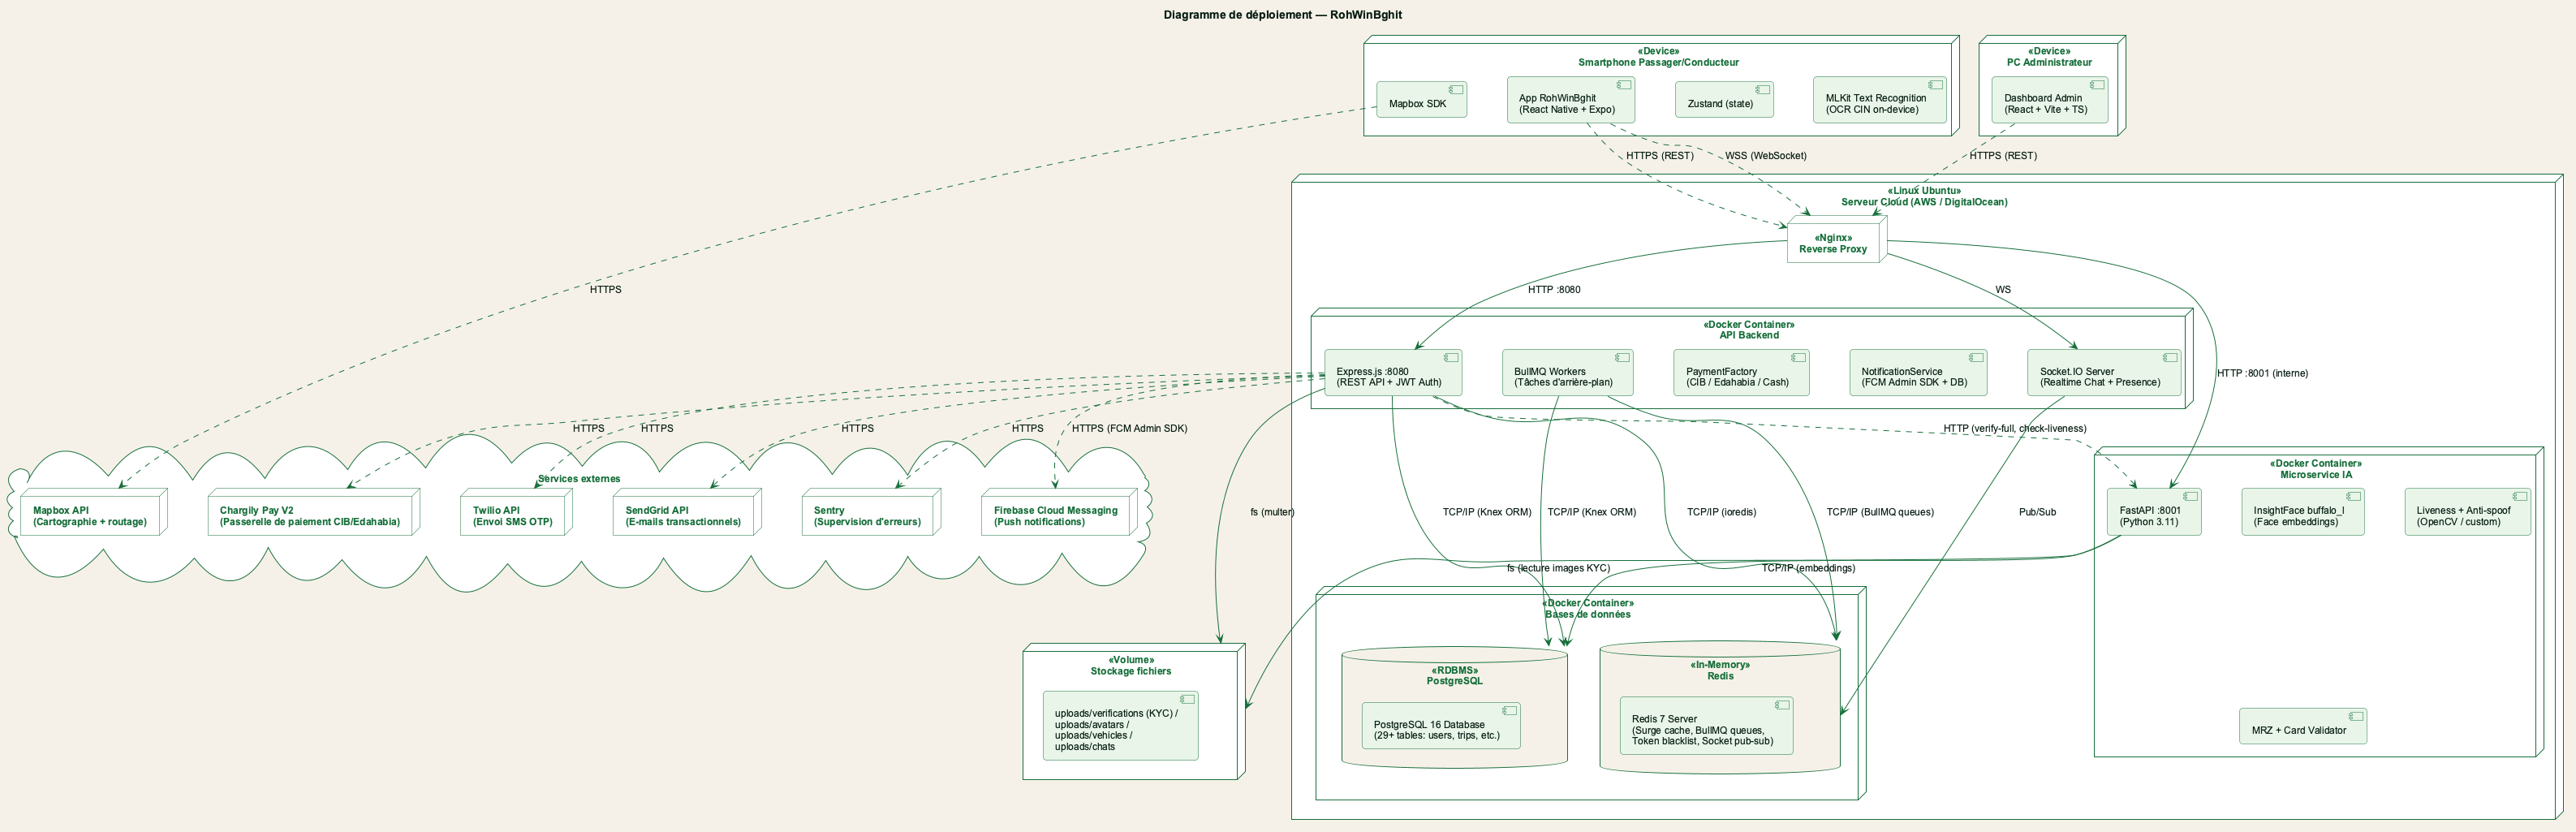
\includegraphics[width=0.95\textwidth]{figures/fig_deployment}
  \caption{Diagramme de déploiement UML~2.5 — RohWinBghit}
  \label{fig:deploiement}
\end{figure}

\subsection{Justification des choix de conception et conformité SOLID}
\label{sec:justification}

\paragraph{Patrons de conception mobilisés.} Le \textit{back-end} suit un découpage en couches inspiré de la \textit{Clean Architecture}. Trois patrons de conception classiques~\cite{gof_design_patterns_1994} sont systématiquement mobilisés~: \textbf{Strategy/Factory} pour le paiement (extensibilité vers Stripe/PayPal), \textbf{Repository} pour l'accès aux données, et \textbf{Observer} pour la diffusion des événements.

\paragraph{Conformité \textsc{solid}.} Chaque module respecte les cinq principes~: SRP par séparation contrôleur/service/dépôt, OCP via les patrons Strategy/Factory, LSP par interfaces explicites, ISP par contrats fins, DIP par injection systématique.

\paragraph{Risques techniques anticipés.} L'analyse des risques techniques critiques inhérents à l'exploitation de la plateforme et les stratégies d'atténuation logicielle associées sont synthétisées dans le tableau~\ref{tab:risques-mitigations}.

\begin{table}[!htbp]
\centering
\small
\renewcommand{\arraystretch}{1.3}
\begin{tabularx}{\textwidth}{|X|c|X|}
\hline
\rowcolor{rohlight}
\textbf{Risque technique identifié} & \textbf{Impact} & \textbf{Stratégie d'atténuation (Mitigation)} \\
\hline
\textbf{Latence réseau} (connexion 3G/4G instable inter-wilayas) & Élevé & Mise en cache locale Redis 7, compression des payloads JSON, et requêtes idempotentes. \\
\hline
\textbf{Faux positifs / négatifs} du pipeline KYC biométrique & Critique & Seuils adaptatifs par rôle et file d'attente de modération manuelle administrative asynchrone. \\
\hline
\textbf{Indisponibilité de la passerelle} de paiement électronique & Élevé & Application du patron Strategy/Factory pour un repli transparent vers le paiement en espèces. \\
\hline
\textbf{Fuite de données biométriques} et personnelles & Critique & Chiffrement AES-256-GCM au repos, purge des pièces d'identité temporaires après validation (conformité Loi 25-11). \\
\hline
\end{tabularx}
\caption{Analyse et stratégies d'atténuation des risques techniques critiques}
\label{tab:risques-mitigations}
\end{table}


\clearpage
\section{Modélisation mathématique de la sécurité KYC}
\label{sec:securite-biometrique}

La modélisation mathématique du pipeline de décision biométrique KYC s'appuie sur trois scores flottants normalisés~:
\begin{itemize}
  \item Le score de conformité d'identité ($S_{id}$), mesurant la corrélation par distance cosinus entre l'embedding facial extrait de la carte d'identité nationale (CIN) et l'embedding extrait de la vidéo par l'architecture ArcFace.
  \item Le score de détection de vivacité ($S_{liv}$), évaluant l'authenticité de la présence physique de l'utilisateur.
  \item Le score d'anti-spoofing ($S_{as}$), détectant la présentation de supports de rejeu (écrans, masques ou impressions papier).
\end{itemize}

Les taux d'erreur du pipeline sont définis selon les métriques internationales d'évaluation de la biométrie~:
\begin{itemize}
  \item \textbf{APCER} (\textit{Attack Presentation Classification Error Rate})~: Taux de classification erronée des présentations d'attaque.
  \item \textbf{BPCER} (\textit{Bona Fide Presentation Classification Error Rate})~: Taux de classification erronée des présentations légitimes.
  \item \textbf{ACER} (\textit{Average Classification Error Rate})~: Taux moyen d'erreur de classification.
\end{itemize}

Ces métriques sont formalisées au moyen des équations mathématiques suivantes~:

\begin{equation}
\text{APCER} = \frac{1}{N_{\text{PA}}} \sum_{i=1}^{N_{\text{PA}}} \text{Res}(i)
\end{equation}

\begin{equation}
\text{BPCER} = \frac{1}{N_{\text{BF}}} \sum_{j=1}^{N_{\text{BF}}} (1 - \text{Res}(j))
\end{equation}

\begin{equation}
\text{ACER} = \frac{\text{APCER} + \text{BPCER}}{2}
\end{equation}

Où $N_{\text{PA}}$ est le nombre de présentations d'attaque soumises lors de l'évaluation, $N_{\text{BF}}$ est le nombre de présentations légitimes, et $\text{Res}(x)$ est la fonction de décision binaire de l'algorithme d'identification, retournant la valeur 1 pour une attaque détectée et 0 pour un enrôlement accepté.

La plateforme adopte une stratégie d'analyse multi-seuils différenciée selon la criticité des rôles~:

\paragraph{Profil Conducteur (Haute criticité)~:}
\begin{equation}
\text{Statut} = \begin{cases} 
\text{Accepté} & \text{si } S_{id} \geq 0{,}65 \wedge S_{liv} \geq 0{,}65 \wedge S_{as} \geq 0{,}60 \\
\text{Rejeté} & \text{si } S_{id} < 0{,}30 \vee S_{liv} < 0{,}30 \\
\text{Revue Manuelle} & \text{sinon}
\end{cases}
\end{equation}

\paragraph{Profil Passager (Criticité moyenne)~:}
\begin{equation}
\text{Statut} = \begin{cases} 
\text{Accepté} & \text{si } S_{id} \geq 0{,}60 \wedge S_{liv} \geq 0{,}55 \wedge S_{as} \geq 0{,}50 \\
\text{Rejeté} & \text{si } S_{id} < 0{,}30 \vee S_{liv} < 0{,}30 \\
\text{Revue Manuelle} & \text{sinon}
\end{cases}
\end{equation}

La synthèse de ces seuils décisionnels configurés pour le microservice d'IA et la file d'attente de revue administrative manuelle selon le rôle de l'utilisateur est présentée dans le tableau~\ref{tab:seuils-biometriques}.

\begin{table}[!htbp]
\centering
\small
\renewcommand{\arraystretch}{1.3}
\begin{tabularx}{\textwidth}{|>{\hsize=1.25\hsize}X|>{\centering\arraybackslash\hsize=0.85\hsize}X|>{\centering\arraybackslash\hsize=0.85\hsize}X|>{\centering\arraybackslash\hsize=0.9\hsize}X|>{\hsize=1.15\hsize\arraybackslash}X|}
\hline
\rowcolor{rohlight}
\textbf{Rôle de l'utilisateur} & \textbf{Identité ($S_{id}$)} & \textbf{Vivacité ($S_{liv}$)} & \textbf{Anti-spoofing ($S_{as}$)} & \textbf{Action de rejet immédiat} \\
\hline
\textbf{Conducteur} (Haute criticité) & $\geq 0{,}65$ & $\geq 0{,}65$ & $\geq 0{,}60$ & Si $S_{id} < 0{,}30$ ou $S_{liv} < 0{,}30$ \\
\hline
\textbf{Passager} (Criticité moyenne) & $\geq 0{,}60$ & $\geq 0{,}55$ & $\geq 0{,}50$ & Si $S_{id} < 0{,}30$ ou $S_{liv} < 0{,}30$ \\
\hline
\end{tabularx}
\caption{Seuils de décision et de classification biométrique KYC par rôle}
\label{tab:seuils-biometriques}
\end{table}

\clearpage
\section{Modélisation dynamique des processus métiers (BPMN)}
\label{sec:bpmn}

La modélisation des processus métier via la notation \textsc{bpmn} (\textit{Business Process Model and Notation}) permet de formaliser la séquence des activités, les flux de messages et les événements décisionnels entre les différents acteurs et la plateforme \textit{RohWinBghit}. Nous détaillons ci-dessous les trois processus métier fondamentaux du système.

\subsection{Processus métier du conducteur}
\label{sec:bpmn-driver}

La figure~\ref{fig:proc-driver} décrit le parcours du conducteur, depuis son inscription et sa vérification d'identité (KYC) jusqu'à la publication de trajets et l'encaissement de ses revenus. Le processus d'inscription d'un conducteur avec mise en attente \textsc{kyc} s'articule comme suit. L'utilisateur saisit son numéro de téléphone et reçoit un code \textsc{otp} par \textsc{sms}. Après validation, il complète son profil personnel puis enregistre son véhicule. Le système initialise alors son statut de vérification à \textit{unverified} et le redirige vers le parcours \textsc{kyc}~: capture du recto et du verso de la carte nationale d'identité, puis capture vidéo de vivacité (3~secondes). Les artefacts sont téléversés de manière asynchrone vers le microservice FastAPI, qui exécute le pipeline d'inférence en quatre étages (extraction \textsc{ocr}, comparaison faciale ArcFace, détection de vivacité, anti-spoofing). Le résultat est une décision à trois états~: si l'ensemble des scores dépasse les seuils conducteur ($S_{\text{facial}} \geq 0{,}65$, $S_{\text{liveness}} \geq 0{,}65$, $S_{\text{antispoof}} \geq 0{,}60$), le statut passe directement à \textit{verified} et le conducteur peut publier des trajets. Si les scores sont intermédiaires, le dossier est placé en file d'attente \textit{pending\_review} pour examen humain par un administrateur. En cas de score inférieur au seuil d'échec critique ($< 0{,}30$), le système enregistre automatiquement un événement de fraude dans la table \texttt{fraud\_events} et rejette la demande.

\begin{figure}[H]
\centering
\resizebox{0.9\textwidth}{!}{%

\includegraphics{fig_driver_process.png}%
}
\caption{Processus métier du conducteur}
\label{fig:proc-driver}
\end{figure}

\subsection{Processus métier du passager}
\label{sec:bpmn-passenger}

La figure~\ref{fig:proc-passenger} illustre le processus de recherche, de réservation et de paiement électronique sécurisé suivi par le passager. Le flux transactionnel de séquestre du paiement électronique obéit à une logique de protection bilatérale. Lorsqu'un passager confirme une réservation et choisit un paiement par carte \textsc{cib} ou \textit{Edahabia}, le montant total est débité du compte du passager via la passerelle \textsc{satim} et immédiatement crédité sur le portefeuille interne de la plateforme (table \texttt{wallets}), et non sur celui du conducteur. Les fonds demeurent en séquestre jusqu'à l'achèvement effectif du trajet. Lorsque le conducteur marque le trajet comme terminé et que le passager ne conteste pas dans un délai de 24~heures, la plateforme libère automatiquement les fonds vers le portefeuille du conducteur, après déduction de la commission de 12\,\%. En cas d'annulation par le conducteur avant le départ, un remboursement intégral est déclenché automatiquement. Ce mécanisme de séquestre élimine le risque de non-prestation tout en sécurisant les revenus de la plateforme.

\begin{figure}[H]
\centering
\resizebox{0.9\textwidth}{!}{%

\includegraphics{fig_passenger_process.png}%
}
\caption{Processus métier du passager}
\label{fig:proc-passenger}
\end{figure}

\subsection{Processus opérationnel de l'administrateur}
\label{sec:bpmn-admin}

La figure~\ref{fig:proc-admin} présente le processus opérationnel de supervision et de modération de la plateforme par l'administrateur. L'administrateur veille à la santé de la plateforme par trois boucles~: la modération continue des contenus, le traitement des litiges et la revue des KYC litigieux. L'administrateur consulte en continu la file d'attente des dossiers en attente de revue (\textit{pending\_review}), examine les pièces justificatives et les scores d'inférence générés par le service d'IA, puis valide ou rejette le dossier en motivant sa décision. En cas de litige signalé par un passager (par exemple, non-présentation du conducteur ou trajet incomplet), l'administrateur analyse les traces du trajet, les échanges de messagerie et les positions GPS enregistrées, puis procède à l'arbitrage en débloquant les fonds vers le conducteur ou en remboursant le passager. Ces processus garantissent la qualité du service offert aux utilisateurs finaux.

\begin{figure}[H]
\centering
\resizebox{0.9\textwidth}{!}{%

\includegraphics{fig_admin_process.png}%
}
\caption{Processus opérationnel de l'administrateur}
\label{fig:proc-admin}
\end{figure}

\clearpage
\section{Modélisation statique du domaine UML}
\label{sec:conception-statique}

Cette section formalise la structure statique du domaine, ainsi que le dictionnaire de ses classes et concepts métiers.

\subsection{Diagramme de classes du domaine}
\label{sec:classes}

La figure~\ref{fig:classes} représente le diagramme global de classes participantes du domaine.

\begin{landscape}
\begin{figure}[!htbp]
\centering

\includegraphics[width=\linewidth,height=0.85\textheight,keepaspectratio]{fig_class_diagram.png}
\caption{Diagramme de classes du domaine (vue conceptuelle)}
\label{fig:classes}
\end{figure}
\end{landscape}

La classe \texttt{User} est modélisée comme classe mère abstraite, avec trois sous-classes concrètes~: \texttt{Passenger}, \texttt{Driver} et \texttt{Admin}. Le domaine s'articule autour de quatre agrégats~:
\begin{enumerate}
  \item \textbf{Agrégat Transport~:} \texttt{Trip}, \texttt{TripRequest}, \texttt{Route}, \texttt{Booking}, \texttt{Vehicle}.
  \item \textbf{Agrégat Paiement~:} \texttt{Payment}, \texttt{Wallet}, \texttt{WalletTransaction}, \texttt{SurgePricingRule}.
  \item \textbf{Agrégat Identité~:} \texttt{IdentityVerification}, \texttt{FaceEmbedding}, \texttt{FraudEvent}.
  \item \textbf{Agrégat Communication~:} \texttt{Chat}, \texttt{Message}, \texttt{Notification}, \texttt{Review}.
\end{enumerate}

Le modèle intègre quatre patrons de conception~: \textit{Strategy} et \textit{Factory} pour les paiements, \textit{Repository} pour l'accès aux données, et \textit{Observer} pour la diffusion des événements.

\begin{landscape}
\subsection{Dictionnaire des classes et concepts métier}
\label{sec:classes-description}

Le tableau~\ref{tab:classes} synthétise les entités principales avec leurs attributs et méthodes métier.

\begin{table}[!htbp]
\centering
\footnotesize
\renewcommand{\arraystretch}{1.3}
\begin{tabularx}{\linewidth}{|l|X|X|}
\hline
\rowcolor{rohlight}
\textbf{Classe} & \textbf{Attributs principaux} & \textbf{Méthodes métier} \\
\hline
\texttt{User} (\textit{Abstraite}) & id, phone, email, firstName, lastName, verificationStatus, createdAt & register(), verifyOtp(), completeKyc() \\
\hline
\texttt{Passenger} & paymentMethods, averagePassengerRating & reserveTrip(), cancelReservation() \\
\hline
\texttt{Driver} & driverScore, vehicleId, verificationId & publishTrip(), manageBooking() \\
\hline
\texttt{Admin} & adminLevel & moderateReview(), reviewKyc() \\
\hline
\texttt{Vehicle} & id, driverId, brand, model, licensePlate, color, seatsAvailable & register(), update(), deactivate() \\
\hline
\texttt{Trip} & id, driverId, vehicleId, originWilayaId, destinationWilayaId, departureAt, pricePerSeat, availableSeats, status & publish(), cancel(), computeSurgePrice() \\
\hline
\texttt{TripRequest} & id, passengerId, fromWilayaCode, toWilayaCode, requestedDate, seats, status & create(), match(), expire() \\
\hline
\texttt{Booking} & id, tripId, passengerId, seats, totalPrice, status, paymentStatus & confirm(), cancel(), generateQr() \\
\hline
\texttt{Payment} & id, bookingId, method, amount, status, transactionRef & process(), refund() \\
\hline
\texttt{IdentityVerification} & id, userId, faceMatchScore, livenessScore, antispoofScore, status, role & submit(), processAI(), reviewManually() \\
\hline
\texttt{FraudEvent} & id, userId, verificationId, eventType, severity & flag(), investigate() \\
\hline
\texttt{Wallet / WalletTransaction} & balance, currency / type, amount, reference & credit(), debit(), record() \\
\hline
\texttt{Chat / Message} & id, tripId, senderId, content, sentAt & send(), markAsRead() \\
\hline
\texttt{Notification} & id, userId, type, title, body & dispatch(), markAsRead() \\
\hline
\texttt{Review} & id, tripId, authorId, targetId, rating & submit(), moderate() \\
\hline
\end{tabularx}
  \caption{Description des classes du domaine}
  \label{tab:classes}
\end{table}
\end{landscape}

\clearpage
\section{Conclusion}

Ce chapitre a présenté les choix méthodologiques et la conception de la solution logicielle. Après avoir détaillé le déroulement des sprints Scrum (section~2.2), nous avons exposé la conception de l'architecture multi-services découplée (section~2.3). La dimension de sécurité et de confiance a été modélisée mathématiquement à travers le pipeline de décision biométrique KYC (section~2.4). Les flux opérationnels de la plateforme ont été décrits en notation BPMN 2.0 (section~2.5) et la structure conceptuelle a été formalisée par le diagramme de classes logiques du domaine (section~2.6). Le chapitre suivant détaille la réalisation technique, la campagne de tests Jest et l'évaluation d'utilisabilité quantitative.
